\documentclass{article} % For LaTeX2e
\usepackage{nips15submit_e,times}
\usepackage{hyperref}
\usepackage{url}
\usepackage{graphicx}
\usepackage{algorithm}  
\usepackage{algorithmic}
\usepackage[colorlinks,linkcolor=blue]{hyperref}
\usepackage{listings}
\usepackage{color}
\usepackage{amssymb}
\usepackage{amsmath}
\usepackage{caption}
\usepackage{subfigure}

\definecolor{dkgreen}{rgb}{0,0.6,0}
\definecolor{gray}{rgb}{0.5,0.5,0.5}
\definecolor{mauve}{rgb}{0.58,0,0.82}

\lstset{frame=tb,
  language=Python,
  aboveskip=3mm,
  belowskip=3mm,
  showstringspaces=false,
  columns=flexible,
  basicstyle={\small\ttfamily},
  numbers=none,
  numberstyle=\tiny\color{gray},
  keywordstyle=\color{blue},
  commentstyle=\color{dkgreen},
  stringstyle=\color{mauve},
  breaklines=true,
  breakatwhitespace=true,
  tabsize=3
}

%\documentstyle[nips14submit_09,times,art10]{article} % For LaTeX 2.09


\title{Weekly Report(July 18th, 2019)
}


\author{
David S.~Hippocampus\thanks{ Use footnote for providing further information
about author (webpage, alternative address)---\emph{not} for acknowledging
funding agencies.} \\
Department of Computer Science\\
Cranberry-Lemon University\\
Pittsburgh, PA 15213 \\
\texttt{hippo@cs.cranberry-lemon.edu} \\
\And
Coauthor \\
Jianghao Lin \\
Shanghai Jiao Tong University \\
\texttt{chiangel.ljh@gmail.com} \\
\AND
Coauthor \\
Affiliation \\
Address \\
\texttt{email} \\
\And
Coauthor \\
Affiliation \\
Address \\
\texttt{email} \\
\And
Coauthor \\
Affiliation \\
Address \\
\texttt{email} \\
(if needed)\\
}

% The \author macro works with any number of authors. There are two commands
% used to separate the names and addresses of multiple authors: \And and \AND.
%
% Using \And between authors leaves it to \LaTeX{} to determine where to break
% the lines. Using \AND forces a linebreak at that point. So, if \LaTeX{}
% puts 3 of 4 authors names on the first line, and the last on the second
% line, try using \AND instead of \And before the third author name.

\newcommand{\fix}{\marginpar{FIX}}
\newcommand{\new}{\marginpar{NEW}}

%\nipsfinalcopy % Uncomment for camera-ready version

\begin{document}


\maketitle

\begin{abstract}
I read the paper \emph{Unsupervised Representation Learning with Deep Convolutional Generative Adversarial Networks} written by Alec Radford in 2016. Also I implement DCGAN on MNIST.
\end{abstract}

\section{Summary of paper DCGANs}

\subsection{Architecture guidelines for stable DCGANs}

\begin{enumerate}
    \item Do not use any pooling layers. Use strided convolutional layers in discriminator network and fractional-strided convolutional layers in generator network instead.
    \item Use batch normalization in both generator and discriminator network. Note that directly applying batch normalization to all layers may result in sample oscillation and instability. In order to avoid this situation, do not apply batch normalization to the output layer of generator and the input layer of discriminator.
    \item Do not use any fully connected layers. We can use global pooling instead which contributes to model stability but slow down the convergence.
    \item Use ReLU activation in generator network for all layers except for the output layer which uses tanh activation to project values to $[-1, 1]$.
    \item Use Leaky ReLU in all layers of discriminator network.
\end{enumerate}

\subsection{Training details for DCGANs}

\begin{enumerate}
    \item No pre-processing. Only use tanh activation to scale the range of value into $[-1,1]$
    \item SGD
    \item Batch size of $128$
    \item All weights are initialized from a zero-center normal distribution with standard deviation $0.02$
    \item The slope of Leaky ReLU is $0.2$
    \item Adam optimizer
    \item Learning rate of $0.0002$
    \item Momentum term $\beta_1$ is $0.5$ instead of $0.9$
\end{enumerate}

\subsection{Validate the model capacity}

In this part, the author mainly measure the capacity of discriminator network as feature extractors compared with other unsupervised learning methods.

\subsubsection{CIFAR dataset}

We use all convolutional layers of discriminator which comes from a pre-trained DCGAN model on Imagenet-1k. We maxpool each layer representation to produce a $4 \times 4$ spatial grid. We then flatten and concatenate these grids to form a $28672$ dimensional vector. By putting the output of the feature vector into a L2-SVM linear model, we can get a classification scores for supervised learning tasks.

As a result, DCGAN+L2-SVM performs better than k-means baseline method but is not as good as the Exemplar CNN(another method to apply unsupervised learning tasks with CNN).

\subsubsection{SVHN dataset}

After the similar approach above, we can transfer the discriminator' convolutional layers into feature vector and put it with L2-SVM. This time, DCGAN+L2-SVM outperform the previous works when labeled data is scarce.

\subsection{Visualization}

In this part, the author wants to mainly validate that the DCGAN model is actually learning features and representation from the image instead of simply memorizing and fitting the input image. The demonstration is various and imaginative.

\subsubsection{Walking in the latent space}

Interpolation applied to latent vector $z$ results in smooth transition on the generated images. E.g. images transfer from having windows to not having windows. This indicates the feature representation in latent vector $z$.

\subsubsection{Visualizing discriminator features}

Using the \emph{guided backpropagation}, we can visualize the last convolutional layer of discriminator network. And we can see many base outline of specific objects like a mirror or a window. This indicates the features learned in discriminator network.

\subsubsection{Visualizing generator features}

The author do the following two experiments, which strongly demonstrate that there is feature hierarchy architecture in generator network.

\begin{enumerate}
    \item \textbf{Eliminate objects by modifying the generator} - Use logistic regression to predict whether a feature activation is on a window or not based on $150$ manually labeled generated images. Drop all activations that are greater than zero(indicating a window). Then, applying the same vector $z$, generator network will produce image without window accordingly! But the generated image is also blurrier.
    \item \textbf{Vector arithmetic} - Applying vector arithmetic on input $z$ will result in feature object combination or elimination.
\end{enumerate}

\section{Implementation of DCGAN on MNIST}

I apply DCGAN on dataset MNIST using PyTorch. By following the architecture guideline and training tutorial in the paper, I think I finally get the generative model converged after 50 epochs training (is that too much?).

The loss of generator and discriminator network are shown in figure \ref{fig:Loss}.

\begin{figure}[h]
	\centering
	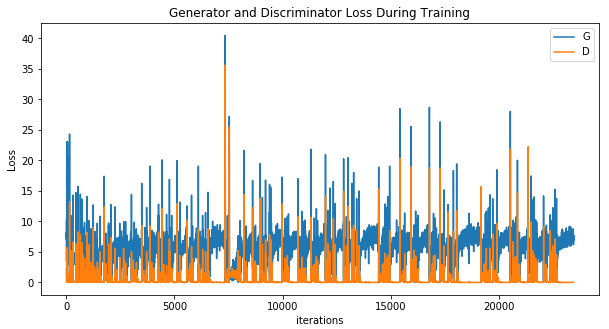
\includegraphics[width=0.9\linewidth]{figures/Loss_of_G_and_D.png}
	\caption{Loss of Generator and Discriminator Network}
	\label{fig:Loss}
\end{figure}

I set a fixed noise input vector to estimate the output of generator during the training. We can clearly see in figure \ref{fig:Output} that the fake image generated from G transfer from the noisy figure to images that indicate numbers.

\begin{figure}[htbp]
\centering
\subfigure[Initial output of Generate Network]{
\begin{minipage}[t]{0.5\linewidth}
\centering
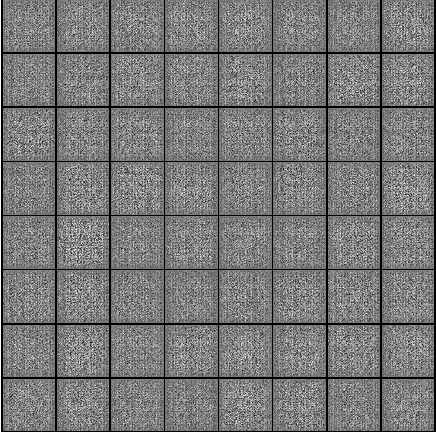
\includegraphics[width=2.5in]{figures/Generated_image_init.png}
%\caption{fig2}
\end{minipage}%
}%
\subfigure[Final output of Generate Network]{
\begin{minipage}[t]{0.5\linewidth}
\centering
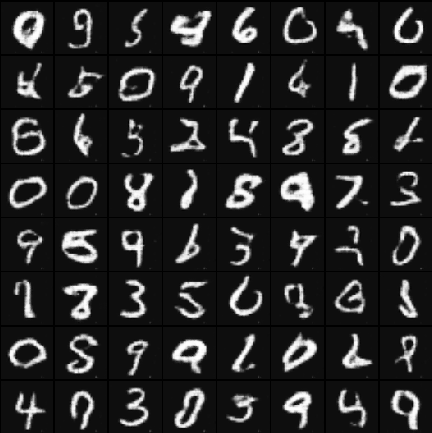
\includegraphics[width=2.5in]{figures/Generated_image_final.png}
%\caption{fig2}
\end{minipage}
}%
\centering
\caption{Output of Generator Network}
\label{fig:Output}
\end{figure}

\end{document}